\capitolo{Dimensionamento e Scelta dei Riduttori}
Con dimensionamento di riduttori si intende la valutazione di aspetti strutturali. La scelta dei riduttori invece coinvolge valutazioni differenti quali dinamiche, di controllo e come si relazionano.

\paragrafo{Come mai i riduttori?}
La scelta di utilizzare riduttori è legata a diversi aspetti:
\begin{enumerate}
    \item Adattamento del campo operativo di motore e carico. Solitamente i motori hanno coppie minori di quelle che sono richieste al carico, mentre possono fornire velocità molto superiori quelle di operazione, in questi casi il riduttore permette di ridurre la velocità e di ottenere una maggior coppia.
    \item Ottimizzazione del sistema. Un riduttore opportunamento scelto permette di ridurre costi, ingombro, consumo energetico e facilitare il controllo
    \item Facilita il controllo. Un riduttore ben scelto permette di linearizzare la dinamica del sistema. Per esempio avendo un carico di momento di inerzia variabile con la posizione, l'uso del riduttore permette di vedere dal motore una $J_{eq}=J_m+J_c\tau_r^2\simeq J_m$, quindi un momento di inerzia minore e circa costante.  
\end{enumerate}

\begin{figure}[h]
    \centering
    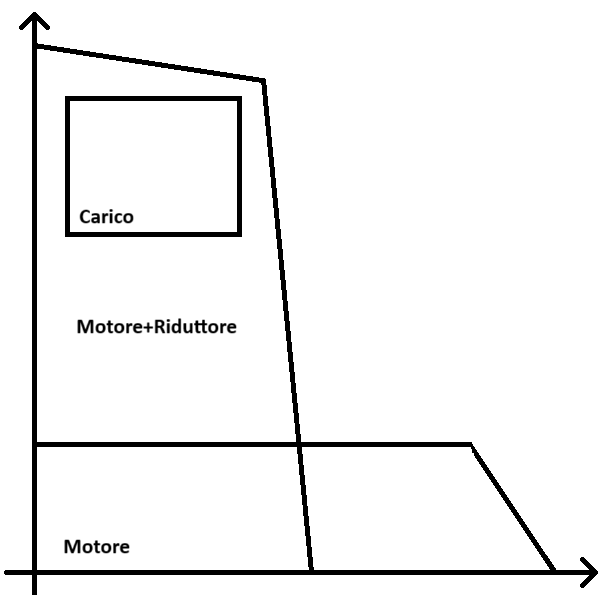
\includegraphics[width=0.2\textwidth]{Immagini/campo_operativo_riduttore.png}
    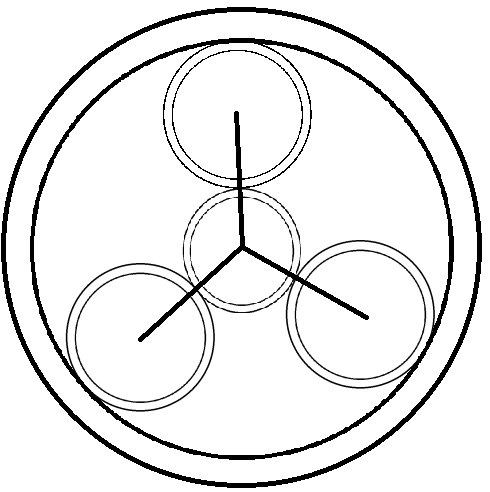
\includegraphics[width=0.18\textwidth,angle=-5]{Immagini/riduttore_epicicloidale.png}
    \caption{Campo operativo (sx), Schema riduttore epicicloidale (dx)}
\end{figure}

\paragrafo{Riduttori Epicicloidali:}
Il riduttore più impiegato nell'industria è quello epicicloidale, questa tipologia è caratterizzata da: buona riduzione; compattezza in termini di rapporto coppia volume; buona distribuzione delle forze; non è invertente; alberi di ingresso e uscita sono coassiali (permettendo una maggior facilità di layout).

\paragrafo{Parametri Progettuali:}
I parametri di progetto di un riduttore noti sono quelli del carico ($J_c$, $C_c$) e legge oraria ($\theta_c(t)$, $\VelAng_c(t)$, $\AccAng_c(t)$); quelli ignoti sono quelli di motore ($J_m$, $C_m$) e riduttore ($\tau_r$, $J_r$, $\eta_r$).
Perciò nel caso di motore riduttore, carico una formulazione più utile, e solitamente usata per determinare la coppia del motore è: 
\[C_m = \left(J_m+J_r\right)\frac{\AccAng_c}{\tau_r} + (C_c + J_c \AccAng_c)\frac{\tau_r}{\eta_r}\]
Il momento di inerzia del riduttore è unione di diversi contributi, ed è fondamentale capire quale sia l'albero a cui è riportato (di solito quello veloce).

\sezione{Step di Dimensionamento}
Per il dimensionamento del riduttore la prima cosa da fare è determinare la taglia, cioè la coppia erogabile $C_r$.
Dipende da considerazioni "strutturali" di tipo normativo\footnote{Non nel senso di legalmente vincolante, più come modo tipico di fare il dimensionamento.} e valutazioni di tipo dinamico (vibrazioni).

\sottosezione{Normativa:}
Il dimensionamento è basato su coppia e velocità, verificando in base al duty cycle la potenza trasmessa dal riduttore per un dato ciclo di riferimento ripetitivo.
In particolare in base al duty cycle vi sono due categorie: 
\begin{itemize}
    \item Regime Intermittente per $<60\%$, per cui occorrono valutazioni su coppia e velocità massime; 
    \item Regime Continuativo per $>60\%$, per cui occorrono valutazioni su coppia e velocità massime e medie.
\end{itemize}
In particolare le valutazioni per coppie e velocità massime andranno effettuate per punti di maggior criticità, ossia la coppia all'albero lento, la velocità all'albero veloce.

\sottosottosezione{Coppia albero lento}
All'albero lento ho la coppia maggiore, quindi è il punto critico. 
Definisco $T_2$ coppia (torque) dell'albero lento (2) la risultante delle coppie applicate sull'albero lento (es coppia e coppia dell'inerzia di carico).
Di $T_2$ è tutto noto, perciò si può procedere subito a questo conto, il cui valore risultante va confrontato con il valore di massima coppia erogata all'albero lento: 
\[1.2\cdot \max{\abs{T_2(t)}}\cdot f_s < T_{2,B}\]
dove:
\begin{itemize}
    \item $1.2$ è un fattore di sicurezza legato alle incertezze di conoscenza dei parametri, valori tipici possono essere $[20\%\div 35\%]$
    \item $f_s$ è un fattore di servizio, valore a catalogo che viene interpretato in modo diverso da ciascun costruttore
    \item $T_{2,B}$ è la coppia massima, è un valore a catalogo e caratterizza la taglia del riduttore. La "B" sta per Bound, in italiano Limite.
\end{itemize}

\paragrafo{Coppia Media:}
Per determinare la coppia media si fa una media cubica ponderata lo spazio di modo che rappresenti la fatica a ciclo variabile, gli effetti termici, calcolata come:
\[
T_{2,media} = \sqrt[3]{\frac{\int^{T_{ciclo}}_0 \abs{T_2^3(t)\VelAng_c(t)}dt}{\int^{T_{ciclo}}_0 \abs{\VelAng_c(t)}dt}}
\]
Anche per questa si va ad applicare un fattore di sicurezza rispetto il punto di funzionamento ottimale $1.2\cdot T_{2,media}<T_{2,nom}$.

\paragrafo{Catalogo:}
Da catalogo COBRA è chiaro come indipendentemente dal numero di stadi la coppia rimanga simile, ed è proprio perché è quella che definisce la taglia. 
Inoltre la maggior parte dei parametri sono simili all'interno di un unica taglia.
Per forti riduzioni (1/10 e 1/100) si nota come le coppie $T_{2,B}$ e $T_{2,N}$ siano differenti tra loro, questo perché la geometria delle ruote saranno molto diverse portando ad avere un ingranamento qualitativamente peggiore.

\sottoparagrafo{Coppia di Arresto:}
La coppia di arresto $T_{2,not}$ è la massima coppia che il riduttore può sopportare in caso di arresto di emergenza (circa 100 volte in vita)\footnote{NB: La coppia di arresto non è quella da usare per la frenata all'interno del ciclo operativo!}.

\sottosottosezione{Velocità all'albero veloce}
Il limite di velocità massima è legato a problemi di sbilanciamento (vedi \ref{sbilanciamentoStat}), ruotando crea una forzante armonica pari alla velocità di rotazione e cresce con velocità e sbilanciamento. 
Deve valere $\max{\VelAng_m(t)}< n_{1,max}$ massima velocità ammissibile, cui aggiungere un fattore di sicurezza.
Diventa problematica non appena $\VelAng \simeq \omega_{N, flessionale}$.
Un aspetto da non sottovalutare è la presenza di eventuali sovraelongazioni nella forma d'onda di velocità legate a controllo reale.
Aumentare la taglia aumenta la massa e la dimensione, perciò aumenta lo sbilanciamento e quindi cala $n_{1,max}$.

\paragrafo{Velocità media all'albero veloce:}
La velocità media deve essere limitata per limitare fenomeni termici e $T_{2,media}$. La velocità media è data dallo spazio totale percorso (in assoluto) su tempo ciclo totale, questo permette di considerare i momenti di arresto marcia in cui il riduttore va a raffreddarsi. La velocità media dev'essere inferiore al valore a catalogo $v_{media} < n_{1,N}$. Anche in questo caso si utilizza un coefficiente di sicurezza del $20\%$. Alcuni costruttori tuttavia usano convenzioni differenti per determinare la velocità media, prestare attenzione alla definizione a catalogo.
Aumentare la taglia aumenta la massa, quindi l'attrito, ossia il calore generato perciò cala anche la $n_{1,N}$, ma in modo poco marcato.

\sottosottosezione{Rapporto di riduzione}
Le velocità sono critiche all'albero veloce, tuttavia $\VelAng_m=\frac{\VelAng_c}{\tau_r}$ di cui a noi è nota solo la velocità del carico. Questo è coerente con il tipo di dimensionamento voluto, perché lo studio di $\tau_r$ si associa ad ulteriori ragionamenti, il vincolo legato a quell'espressione sarà usato per fare una ottimizzazione vincolata.

\paragrafo{Velocità massima all'albero veloce:}
$n_{1,max}>\max{\VelAng_m(t)}$, che in termini di rapporto di velocità diventa $\tau_r>\frac{\max{\VelAng_c}}{n_{1,max}}$.

\paragrafo{Velocità media all'albero veloce:}
$n_{1,N}>\VelAng_m^{media}$, che in termini di rapporto di velocità diventa $\tau_r > \frac{\VelAng_c^{media}}{n_{1,N}}$.

\paragrafo{Velocità limite:}
Tuttavia anche in queste ultime disequazioni è nota la velocità di carico, per le velocità limite bisogna considerare di aver già determinato la coppia, quindi la taglia del riduttore, da cui posso determinare dei valori di velocità limite che saranno abbastanza simili a quelli poi usati effettivamente.

\sottoparagrafo{Se la taglia di quel costruttore non ha valori che vadano bene?}
Se la taglia del costruttore disponibile ha valori di velocità che non sono compatibili con quelli richiesti: per la velocità media c'è poco da fare, nel senso che è determinata dalla legge oraria, cioè dal tipo di funzionalità richiesta e variarla significa non dare al cliente ciò che ha richiesto.
Potrebbe essere possibile modificare il coefficiente di sicurezza di modo da rientrare nella taglia inferiore di riduttore disponibile, ma va fatto coscienti del significato delle implicazioni: la velocità media, moltiplicata la coppia media $T_{2,media}$, è la potenza media $W_{media}$, usata per fare valutazioni termiche, che devono essere rispettate.
Per la velocità massima invece c'è più margine di scelta perché il coefficiente di sicurezza è maggiore. \label{rivalutazione_coeff_sic}

\sottosezione{Valutazioni su Riduttore}
Ci sono diversi aspetti strutturali da considerare per la scelta di un riduttore.

\sottosottosezione{Dimensione dei vari stadi in un multistadio:}
In un riduttore multistadio le dimensioni dei singoli stadi non sono le stesse, perché le coppie che devono sopportare sono differenti, perciò non è esattamente come considerare due singolo stadio.

\sottosottosezione{Massa}
La massa del riduttore è proporzionale alla taglia e al numero di stadi. 
In generale maggiore massa comporta un maggior costo, nonostante ciò l'uso di multistadio può portare un calo del costo del motore e quindi dell'energia (vedi lezione su $\tau$ ottimo).

\sottosottosezione{Momento di inerzia dell'albero veloce}
All'interno di una stessa taglia i valori di inerzia sono molto simili perché le ruote hanno modulo di denti e sezioni sugli alberi simili se non identici, quindi la massa nonché l'inerzia saranno circa uguali.
Le differenze sono legate alle dimensioni delle ruote quindi satelliti e sole, dove il sole porta ad avere un momento di inerzia leggermente maggiore, quindi $J_{1/10}<J_{1/3}$.
Tra le varie taglie invece il momento di inerzia aumenta in modo è più che lineare, quasi quadratico.
A parità di taglia, per diverso numero di stadi, nonostante la massa aumenti nel multistadio, il momento di inerzia cala, perché va considerata l'inerzia equivalente all'albero veloce, quindi: $J_r=J_{1st}+J_{2st}\tau_{1st}^2$.

\begin{figure}[h]
    \centering
    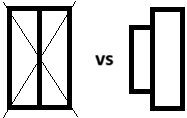
\includegraphics[width=0.15\textwidth]{Immagini/ridutt_2st_diff_dim.png}
    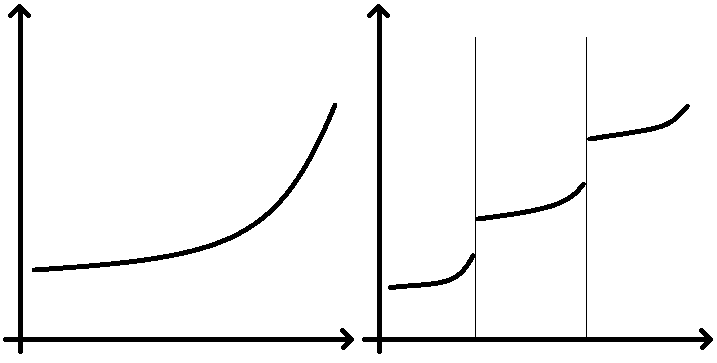
\includegraphics[width=0.35\textwidth]{Immagini/momento_inerzia_stadi.png}
    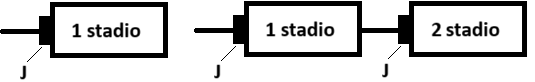
\includegraphics[width=0.4\textwidth]{Immagini/momento_inerzia_albero_veloce.png}
    \caption{Riduttori bistadio (sx); Grafici inerzia (centro); Schema equivalente inerzia (dx)}
\end{figure}

\sottosottosezione{Rendimento}
Il rendimento varia con l'aumentare del numero di stadi, perché $\eta_r=\Pi_i \eta_i$, valori tipici sono:
\begin{itemize}
    \item 1 stadio: $96\% \div 98\%$
    \item 2 stadio: $94\% \div 95\%$
    \item 3 stadio: $90\% \div 92\%$
\end{itemize}
I valori vengono presi in condizioni nominali, il rendimento è una curva che dipende dal punto di lavoro.

\sottosottosezione{Rigidezza}
In condizioni ideali bloccare l'albero veloce comporta il blocco dell'albero lento, tuttavia in condizioni reali presenterà una variazione circa lineare di tipo elastico (soprattutto nella zona di lavoro), a cui si va ad aggiungere una componente non lineare legata al gioco.
Perciò può essere introdotto un nuovo modello per il riduttore che consideri la rigidezza reale considerandolo come una molla.
Il sistema passa ad avere due gradi di libertà, non è più valida l'espressione $\VelAng_m \neq \frac{\VelAng_c}{\tau_r}$, ma diventerà, considerando $T(s)$ funzione di trasferimento:
\[s \theta_c(s)=s \theta_m \tau_r T(s)\]
Nel caso multistadio la rigidezza da considerare è una rigidezza equivalente data dalla serie, perciò sarà minore delle rigidezze dei singoli stadi: $K_r=\frac{1}{\frac{\tau_2^2}{k_1}+\frac{1}{k_2}}<k_1,k_2$.

\begin{figure}[h]
    \centering
    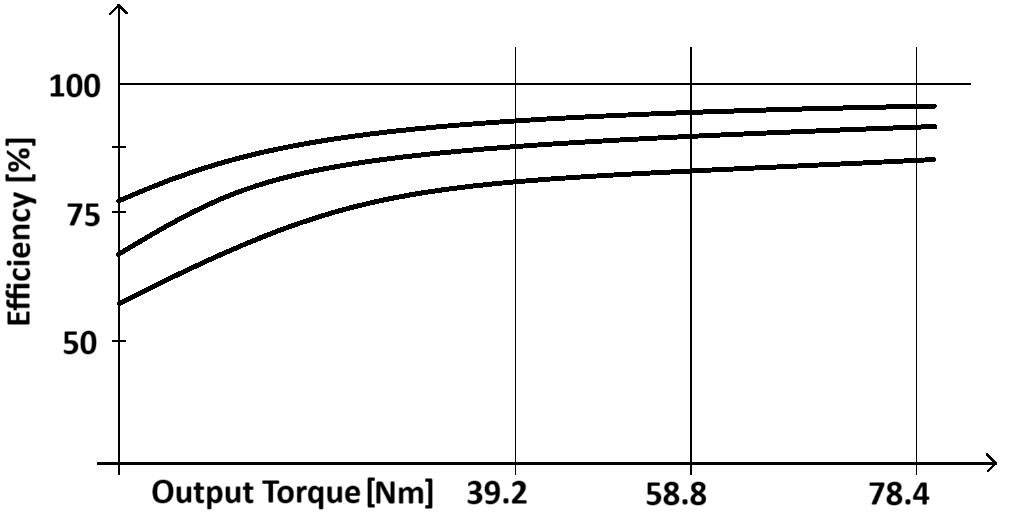
\includegraphics[width=0.4\textwidth]{Immagini/efficiency_torque.png}
    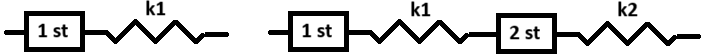
\includegraphics[width=0.5\textwidth]{Immagini/rigidezza_1_2_stadi.png}
    \caption{Caratteristica esempio rendimento sx; Schema equivalente rigidezza dx}
\end{figure}


\paragrafo{Cataloghi:}
Nei cataloghi la rigidezza è definita all'albero lento, perché permette di fare calcoli più semplici in termini di deformazione vista dal carico.
Nel caso del costruttore visto a lezione $k=R_d$, si nota come aumenti con la taglia in modo circa lineare, perché aumentare la sezione e massa del riduttore aumenta la resistenza torsionale. \footnote{Esistono riduttori epicicloidali con rigidezze particolarmente elevate sfruttando una rivisitazione dei riduttori epicicloidali classici, vedi: Galaxie della Wittenstein e Cyclodrive della Sumimoto.}

\sottosottosezione{Gioco}
Il gioco (o backlash) nei riduttori è lo spazio tra dente e dente nella circonferenza primitiva. Il gioco è legato alla dimensione del vano della ruota e dalla dimensione del dente, dipende soprattutto dalla tolleranza che ha la lavorazione.
Si misura in arcmin, dove $1'=\frac{1}{60}^°$.
Può portare a una ridotta precisione, accuratezza o a micro-urti causa di vibrazioni o usura. 

Nei cataloghi il gioco viene valutato all'albero lento (2) per dare un'idea di quanto possa influenzare lo spostamento nel carico, tuttavia agiscono diversi fattori.\footnote{Non è detto che il gioco effettivo sia quello di catalogo, perché c'è dipendenza anche dal controllo. Occorreranno fare approfondite valutazioni in un secondo momento.}

\paragrafo{Posizioni dei denti:}
Ci sono due possibilità di contatto tra i denti, in entrambi i casi avviene in un punto, che varia istante per istante, e che garantisce lo scambio di forze, quindi è presente l'accoppiamento e vale $J_{eq}=J_m+\tau_r^2 J_c$. 
Tuttavia è possibile che non vi sia alcun contatto tra i denti, in questo caso non ci sarebbe nè scambio di forze nè accoppiamento, in questa condizione vale $J_{eq}=J_m$, complicando il controllo, perché può risultare essere elemento di instabilità o di semplice stabilità.

\begin{figure}[h]
    \centering
    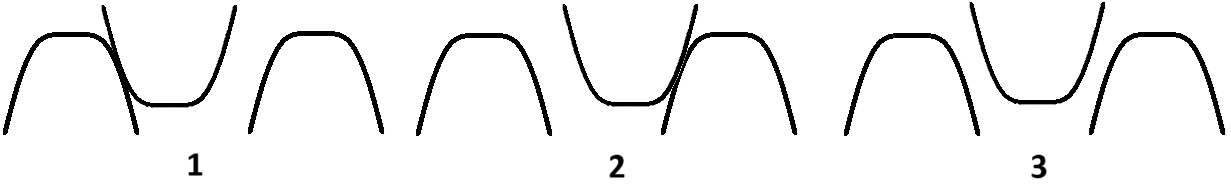
\includegraphics[width=0.5\textwidth]{Immagini/config_denti_gioco.png}
    \caption{1 - Contatto sx; 2 - Contatto dx; 3 - No contatto}
\end{figure}

\paragrafo{Multistadio:}
Il gioco nei riduttori multistadio viene calcolato come valore a catalogo a partire da uno spostamento sull'albero veloce, da riportare sull'albero lento noti i giochi dei singoli stadi, perciò \( \Delta \theta_{out} = \tau_1\tau_2\Delta \theta_{in} + \epsilon_2 +\tau_2\epsilon_1 \), ossia il gioco aumenta con l'aumentare degli stadi.

\paragrafo{Catalogo Wittenstein:}
Confronto catalogo Wittenstein standard e alte performance. In alcuni dei riduttori ad alto performance viene raggiunto gioco nullo, tuttavia non è sempre la soluzione ideale perché non avere gioco significa mantenere un maggiore contatto, quindi aumenta l'attrito. Significa anche che deve aumentare la manutenzione per evitare che polveri si infilino tra le ruote e che vi sia una opportuna lubrificazione. 
Il valore del gioco viene proposto come disuguaglianza in cui il valore viene garantito sotto un massimo.
La vita utile dei riduttori è determinata soprattutto dai cuscinetti che vanno sostituiti a determinati intervalli.

\sottosottosezione{Riduttori epicicloidali di nuovo tipo}
L'obiettivo di riduttori epicicloidali di nuova tipologia è quello di ottenere ridotto (nullo) gioco e elevata rigidezza.
\begin{itemize}
    \item Cyclodrive: \( \tau_r \downarrow \), gioco 0, \( T_2 \uparrow \), \( K \uparrow \), \( \frac{T_2}{V} \) rapporto coppia volume buono, \( \eta_r \downarrow \) rendimento inferiore ai normali epicicloidali, per progetti di fascia alta.
    \item Harmonic Drive: \( \tau_r \downarrow \), gioco 0, \( \eta_r \downarrow \), rigidezza \( \downarrow \) rigidezza ridotta perché il moto è trasmesso da una parte flessibile che ingrana su una fissa. Utilizzata nella robotica collaborativa in cui le velocità sono ridotte e la flessibilità è una specifica.
    \item Galaxie Drive: \( \tau_r \downarrow\downarrow\), \( K \uparrow\uparrow \), \( T_2 \), gioco 0, \( \eta_r \uparrow \), per progetti di fascia alta.
\end{itemize}\label{riduttori_speciali}

\import{Sottofile/}{EsDimRiduttori}

\sezione{Rapporto di Trasmissione Ottimo} \label{tau_ottimo}
Per ricavare il rapporto di trasmissione ottimo si utilizza una ottimizzazione a cui vanno associati ragionamenti aggiuntivi.

Nel caso di sistema motore + riduttore + carico vale la solita relazione \(C_m = (J_m+J_r)\frac{\AccAng_c}{\tau_r} + \tau_r \frac{T_2}{\eta_r}\), dove \((J_m+J_r)\frac{\AccAng_c}{\tau_r}\) è il contributo relativo l'albero veloce mentre \(\tau_r \frac{T_2}{\eta_r}\) è quello relativo l'albero lento.

\begin{figure}[h]
    \centering
    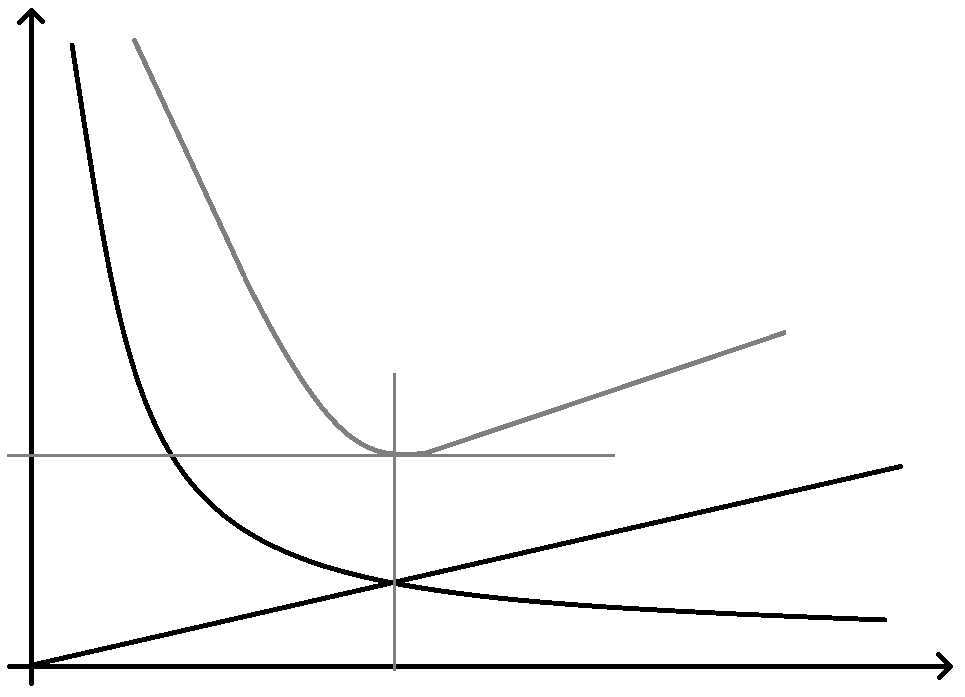
\includegraphics[width=0.4\textwidth]{Immagini/CoppiaTauRott.png}
    \caption{Rapporto di trasmissione ottimo}
\end{figure}


Per quell'espressione di coppia del motore è possibile ricavare il valore ottimo di rapporto di trasmissione \(\tau_{opt}\) di \(\tau_r\) tale che \(\minOtt{C_m}\), ossia \(\derivataparz{C_m}{\tau_r} = 0\), per cui vale:
\[ \tau_{opt} = \sqrt{\eta_r \frac{J_m + J_r}{T_2}\AccAng_c} \]
Per cui è importante notare che \(\eta_r, T_2, \AccAng_c\) sono tempo dipendenti, perciò anche il valore ottimo. In termini matematici ha senso, tuttavia per il progetto occorre avere un numero.
Delle grandezze temporali vanno considerati dei valori "medi" in particolare i valori RMS.

\sottosezione{Valutazioni sulla Coppia}
Parto dal considerare la coppia del motore RMS \(C_m^{RMS} = \sqrt{\frac{\int_0^{T_c} C_m^2(t)dt}{T_c}}\), scelta perchè minimizzare \(C_m\) significa minimizzare la taglia e quindi il costo di un motore.

\sottosottosezione{Caratteristica}
Dalla tipica caratteristica del motore PMSM (brushless) sono evidenti le zone di lavoro continuativo e intermittente.
Si può definire inoltre la \(T_{CS}\) ossia la Coppia Continuativa di Stallo (Torque Continuos Stall) punto per velocità nulla e coppia non nulla massima affinchè funzioni in regime continuativo. Inoltre la \(T_{CS}\) definisce la taglia del motore.

\(T_{CS}\) ha implicazioni per diversi parametri:
\begin{itemize}
    \item Massa cresce linearmente. In base alla famiglia, quindi alla tecnologia costruttiva, ci sono diverse curve.
    \item Costo cresce linearmente. In base alla famiglia, quindi alla tecnologia costruttiva, ci sono diverse curve.
    \item Inerzia cresce più che linearmente, quasi quadraticamente. In base alla geometria dell'albero quindi dal raggio e dalla lunghezza l'inerzia aumenta. La relazione è \(J_{cilindro} = \frac{1}{2} \rho L \pi R^4\)
    \item Attrito cresce linearmente\footnote{Guardare analisi di catalogo Parker.}
\end{itemize}

\paragrafo{Relazione Coppia di Stallo e Coppia RMS:}
Nella fase di dimensionamento di un motore si devono unire la curva caratteristica del motore  e ciclo di riferimento, quindi verificare che il ciclo di lavoro sia composto da punti interni l'area di lavoro e che \(\left(C_m^{RMS},\VelAng_m^{RMS} \right)\) sia interno all'area di lavoro continuativa.
Quest'ultima si traduce in \(C_m^{RMS} < T_{CS}\) e quindi \(\minOtt{C_m^{RMS}}\) implica \(\minOtt{T_{CS}}\).
\begin{figure}[h]
    \centering
    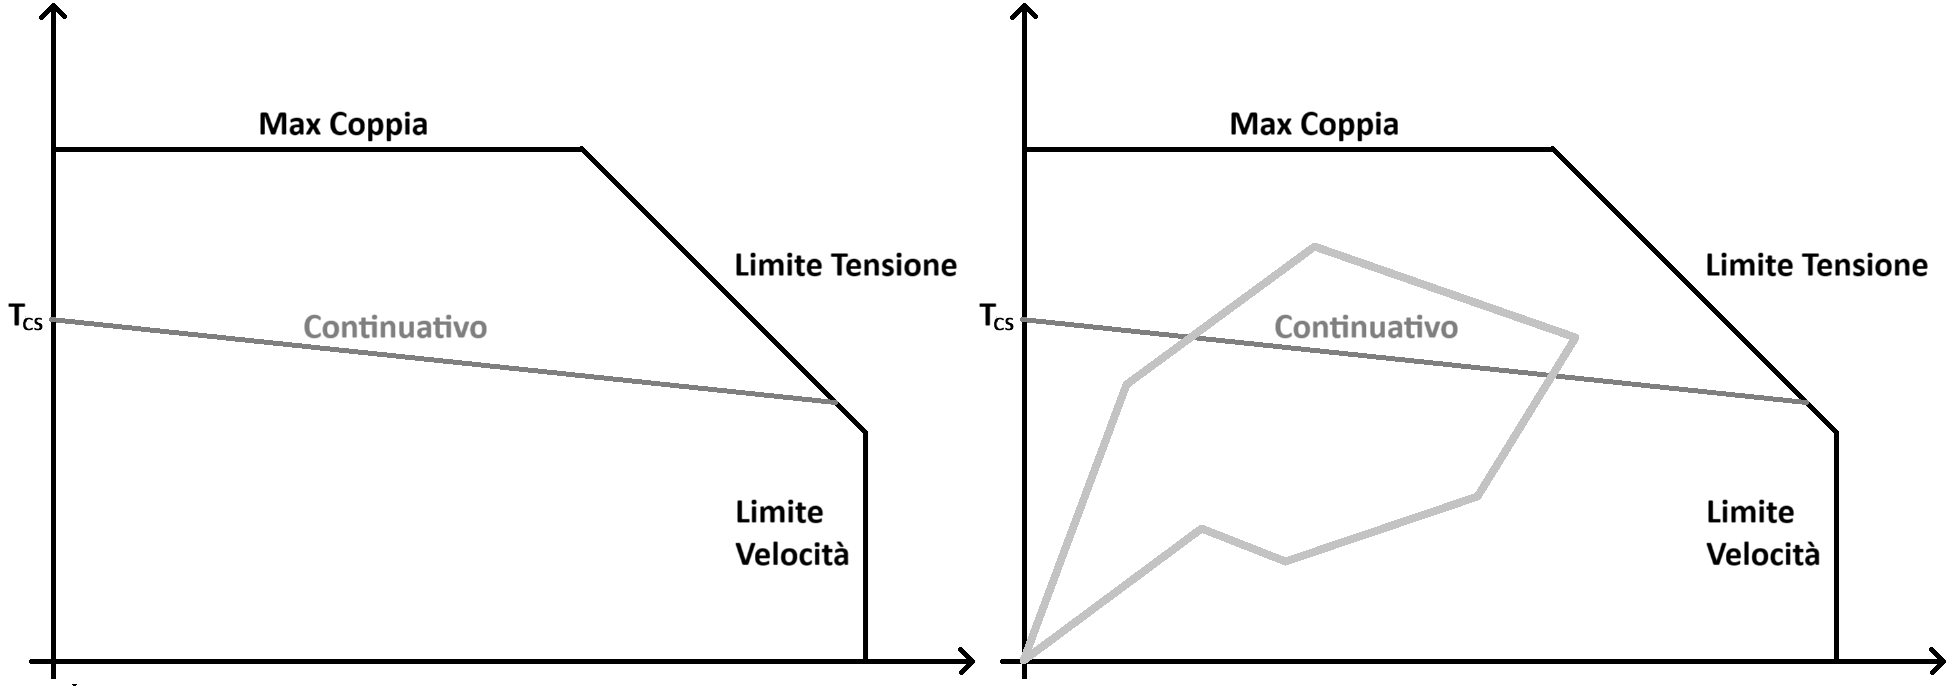
\includegraphics[width=0.6\textwidth]{Immagini/CaratteristicaPMSM.png}
    \caption{Caratteristica di PMSM con ciclo di lavoro}
\end{figure}

\sottosottosezione{Riformulazione con grandezze RMS}
Se si utilizzano le grandezze RMS la riformulazione risulta \(\tau_{opt} = \sqrt{\frac{J_m + J_r}{\left(T_2/\eta_r\right)^{RMS}}\AccAng_c^{RMS}}\). Considerando un rendimento alto, e che comunque il valore ottenuto dovrà essere adattato a quelli presenti nel catalogo disponibile, si può omettere il rendimento, si ottiene quindi un espressione indicativa per la scelta del \(\tau_r\):
\[\tau_{opt} = \sqrt{\frac{J_m + J_r}{T_2^{RMS}}\AccAng_c^{RMS}}\] 

\sottosottosezione{Vincoli}
Finora l'analisi non considerava i vincoli sulla scelta di rapporto di trasmissione.

\paragrafo{Rapporto di Tramsissione Minimo:}
A limiti in termini di \(n_{1,max},n_{1N}\) si associa un vincolo di rapporto di trasmissione minimo \(\tau_{min}\), valori inferiori sono esclusi, questo potrebbe includere anche \(\tau_{ott}^l\), libero; in questo caso \(\tau^\text{vinc}_{ott} = \tau_{min}\) ossia il rapporto di trasmissione ottimo del sistema vincolato diventa il rapporto di trasmissione minimo\footnote{In modo simile a quanto visto per l'esercizio a pagina \pageref{EsercizioDimRid}.}.

\paragrafo{Rapporto di Trasmissione Massimo:}
I vincoli di rapporto di trasmissione massimo sono legati a diversi aspetti.

\begin{enumerate}
    \item Risoluzione del trasduttore di posizione del motore riportato al carico, in particolare, detta \(\delta \theta_m\) risoluzione lato motore, \(\delta \theta_c = \delta \theta_m \tau_r\) ossia \(\tau_r\) piccolo permette di aumentare la risoluzione del carico, a discapito però di un calo della ripetibilità (precisione).
    \item Propagazione dell'errore di posizionamento del motore, in particolare detto \(\epsilon_m\) errore di posizione lato motore, riportato al carico diventa \(\epsilon_c=\epsilon_m \tau_r\), perciò migliora per \(\tau_r\) piccolo.
    \item Limite superiore al rapporto di inerzia \(\rho \) che è il rapporto tra la sommatoria dei momenti di inerzia lato carico riportati al motore su la sommatoria dei momenti di inerzia dell'albero motore. Nel caso in esame di motore riduttore e carico sarebbe\footnote{Nota bene che in realtà \(J_r\) andrebbe ripartita tra contributi di albero lento e albero veloce, tuttavia non sono noti.} \(\rho=\frac{J_c \tau_r^2}{J_m+J_r}\).
    Per \(\rho\) grande diventa più complicato il controllo del sistema in presenza di gioco o elasticità, viene quindi posto un \(\rho_{max}\) che si traduce in una limitazione del \(\tau_r\).
\end{enumerate}

In modo del tutto simile al caso di \(\tau_{min}\), anche il \(\tau_{max}\) potrebbe essere tanto stringente da escludere il valore \(\tau_{opt}^l\), libero, quindi se come in precedenza fosse necessario escluderlo occorrerebbe considerare un rapporto di trasmissione ottimo vincolato \(\tau_{opt}^v=\tau_{max}\).

\begin{figure}[h]
    \centering
    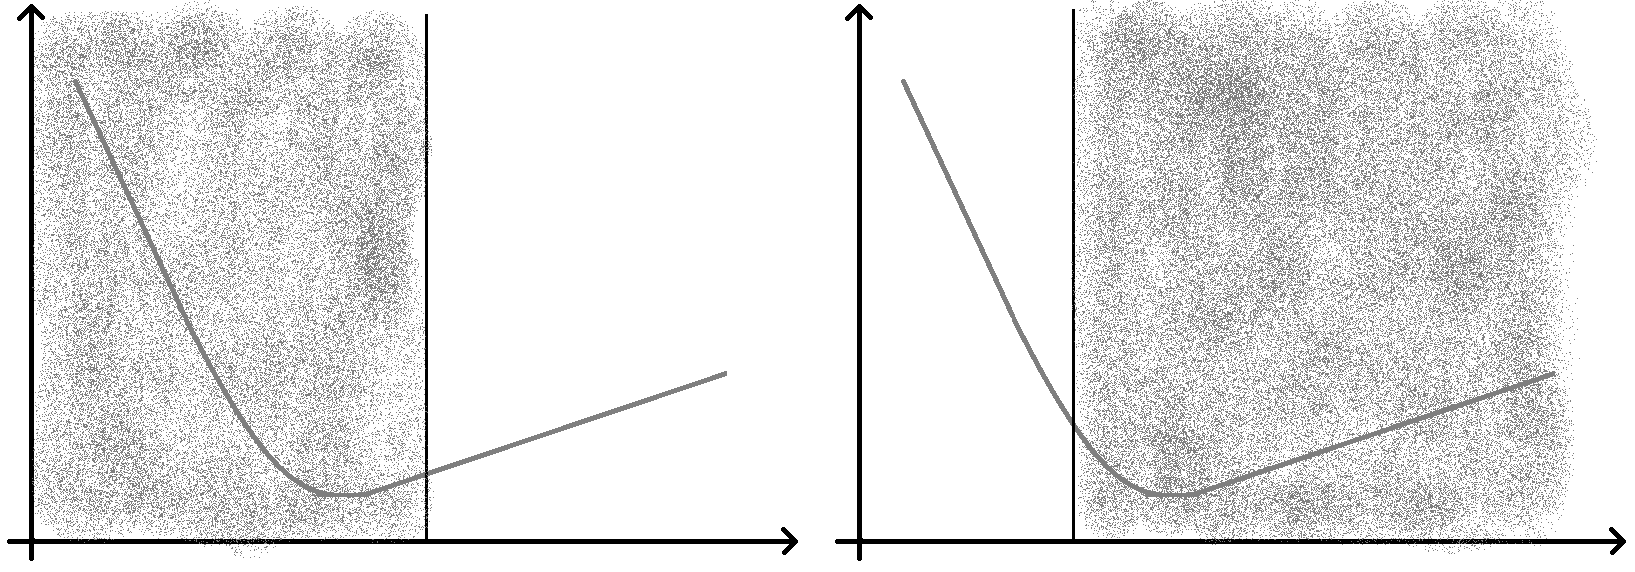
\includegraphics[width=0.6\textwidth]{Immagini/tauRmax_tauRmin.png}
    \caption{Rapporti di trasmissione: minimo sx, massimo dx}
\end{figure}


\sottosezione{Energia Elettrica Assorbita}
L'energia elettrica assorbita è pari a \(E_m = \int^{T_c}_0 v(t) i(t) dt\),  considerando \(i(t)=\frac{C_m}{K_T}\) e \(v(t) = R i(t) + K_B \VelAng_m\), facendo opportune sostituzioni e manipolazione, si ottiene:
\[ E_m = \frac{R}{K_T^2} T_c (C^{RMS}_m)^2 + \frac{K_B}{K_T} \int^{T_c}_0 C_m\VelAng_m dt \]
Dove il primo dei due contributi tendenzialmente è dominante; occorre tuttavia tenere conto del secondo contributo che dipende dalla velocità e che quindi potrebbe diventare più rilevante.
Da queste valutazioni si trova che \(\minOtt{C_m^{RMS}}\) è simile a \(\minOtt{E_m}\), ma il rapporto di trasmissione ottimo per l'energia tendenzialmente è maggiore di quello per la coppia, perciò conviene utilizzare \(\tau_r >\) maggiori.

\sottosezione{Velocità del Motore}
La velocità del motore è inversamente proporzionale al rapporto di trasmissione, quindi per ottenere velocità inferiori conviene utilizzare \(\tau_r >\) maggiori.
Per velocità di motore elevate aumenta la coppia legata all'attrito viscoso; inoltre per velocità elevate \(K_T\) è ridotto, perciò la produzione di coppia richiede maggior corrente, quindi maggiori costi in termini di convertitori.

\sottosottosezione{Attrito viscoso}
Il contributo dell'attrito viscoso si vede all'albero veloce \(C_m = (J_m+J_r)\frac{\AccAng_c}{\tau_r} + f_v \frac{\VelAng_c}{\tau_r}\), che quindi rientra nell'espressione del rapporto di trasmissione ottimo\footnote{Nota bene che \(RMS\{A+B\}\leqslant RMS\{A\} +RMS\{B\}\).} \(\tau_{opt} = \sqrt{\frac{\left[(J_m + J_r)\AccAng_c+f_v \VelAng_c\right]^{RMS}}{\left(T_2/\eta_r\right)^{RMS}}}\), dove \(\VelAng_m\) "alta" porta a \(\tau_r\) "bassi", quindi l'effetto di attrito è maggiore per la zona sinistra del grafico. Vengono favoriti \(\tau_r\) maggiori.

\sottosottosezione{Costante di Coppia}
A parità di taglia del motore, una velocità maggiore porta ad avere \(K_T\) inferiore, perciò il costo della coppia in termini di corrente è superiore. Vengono favoriti \(\tau_r\) maggiori.
Occorre quindi scegliere opportunamente la velocità massima al carico (valutazioni su legge di moto) e il rapporto di trasmissione.

\sottosottosezione{Numero di Stadi}
La scelta del numero di stadi porta ad una serie di valutazioni su rigidezza, gioco, rendimento, inerzia e costo.
In generale la scelta tende comunque a favorire \(\tau_r\) maggiori anche in questo caso.

\begin{figure}[h]
    \centering
    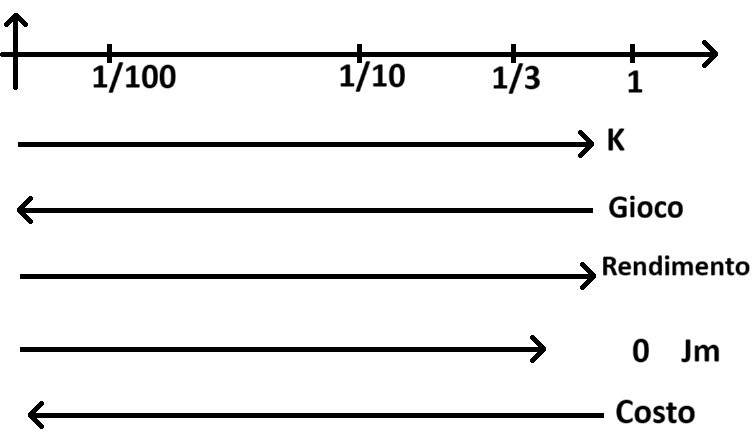
\includegraphics[width=0.4\textwidth]{Immagini/numero_std_rid_tau_opt.png}
    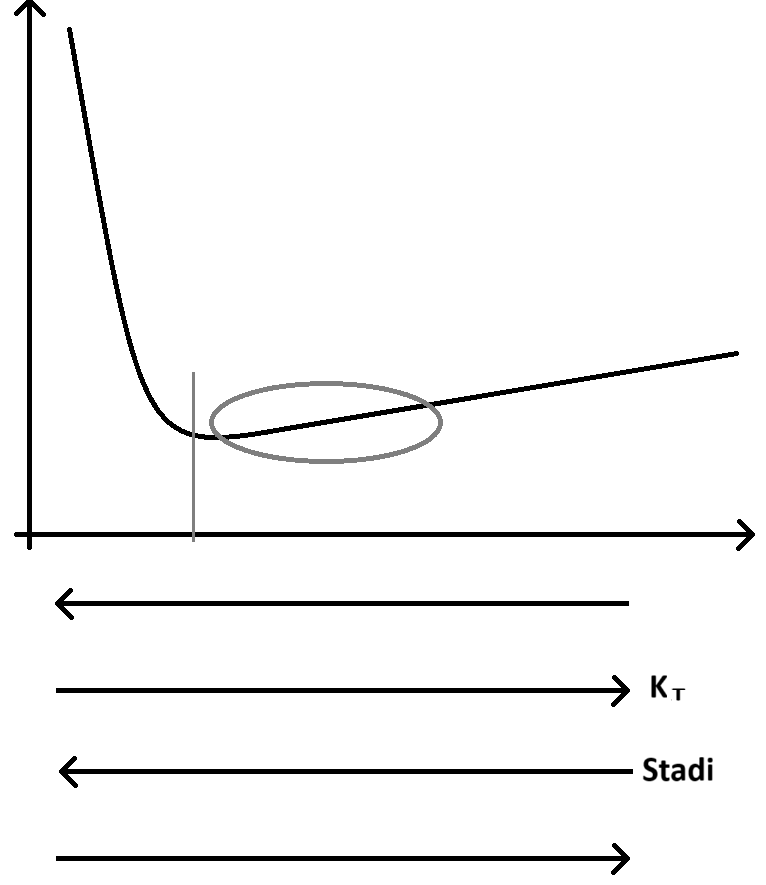
\includegraphics[width=0.4\textwidth]{Immagini/riepilogo_tau_opt.png}
    \caption{Valutazioni per numero di stadi sx; Riepilogo dx}
\end{figure}

\sottosezione{Limite alla Conoscenza dei Valori}
Nella formula del rapporto di trasmissione ottimo  \(\tau_{opt} = \sqrt{\frac{J_m + J_r}{\left(T_2/\eta_r\right)^{RMS}}\AccAng_c^{RMS}}\), dei parametri presenti:
\begin{itemize}
    \item \(T_2, \AccAng_c^{RMS}\) sono indipendenti da \(\tau_r\)
    \item \(\eta\) è dipendente da \(\tau_r\), ma se le differenze sono ridotte si può trascurare
    \item \(J_r\) dipende dalla \(\tau_r\), tuttavia la dipendenza maggiore la ha per la taglia, quindi scelta quella si può scegliere un valore medio o significativo
    \item \(J_m\) dipende da \(T_{CS}\), che a sua volta dipende da \(C_m^{RMS}\) che è legata a \(\tau_r\)
\end{itemize}

Questo problema ha per soluzioni: Utilizzo di metodi di stima; Esperienza; Iterazioni utilizzando buon senso.